%!TEX root = paper.tex
\chapter{The pipeline}
\label{sec:overview}

\begin{figure}
\center\includegraphics{diagrams/pipeline.pdf}
\caption{Diagram of the pipeline}\label{fig:pipeline}
\end{figure}

\begin{figure}
\begin{mdframed}
\begin{description}
    \item[Source component]
        The smallest unit of user-written source which can have its
        dependencies resolved, e.g., a library, an executable or a test
        suite.  A \textbf{source package} contains one or more source
        components, and is the unit of code that may be distributed
        (e.g., on Hackage).  A source package is identified by a
        \textbf{package identifier} consisting of a package name and
        package version (e.g., \verb|p-0.1|); a source component is in
        turn identified by a \textbf{source component identitifer}
        consisting of the package identifier with the name of the
        component.
    \item[\Ccomp{}] ($\Scomp$ in Figure~\ref{fig:rcomponents}) The output of dependency
        resolution on a source component.  A \ccomp{} is the
        input source with direct dependencies resolved to
        other \ccomp{}s, and \Backpack{}-irrelevant Cabal fields dropped.
        As dependency resolution is
        nondeterministic, a \ccomp{} is identified by a \textbf{\cid}
        ($p$), which augments the source component identifier with the
        resolved \cid{}s of the direct dependencies.  (Thus, the \cid{}
        identifies the entire transitive source a component depends on.)
        In \Backpack{}, we treat \cid{}s as opaque strings.
    \item[\Unit{}] ($\Uunit$ in Figure~\ref{fig:lcomponents}) The output
        of mixin linking on a \ccomp{}, where we have computed the ``wiring
        diagram'' for the direct dependencies of the unit, describing how
        requirements of the \ccomp{}'s direct dependencies have been
        (partially) filled.  Mixin linking is
        deterministic; thus, a \unit{} is also identified by a \cid{}.  A
        \unit{} can be typechecked by the compiler.
%   \item[Instantiated component]  The output of instantiating a
%       \unit{}.  It is identified by an \textbf{\uid{}} ($P, Q ::= \I{p}[S]$,
%       also known as a \emph{unit identifier})
%       which is simply a \cid{} equipped with a module substitution.
%       If the substitution has no module holes, an instantiated component
%       can be compiled; otherwise, the type of an instantiated component
%       can be computed by appropriately substituting over the type of the \unit{}.  Two types are equivalent if and only if
%       they are defined by the same module from the same \unit{}s instantiated in the same
%       way.
%   \item[Module substitution] ($S ::= \overline{m \mapsto M}$)  A module substitution
%       is a mapping from module names to module identifiers.  These are most
%       commonly used to say how a component is instantiated.
%   \item[Module name] ($m$) Source-level module name, e.g., \verb|Data.Map|.
%   \item[Module identifier] ($M ::= P\!:\!m \,|\, \holevar{m}$)  A fully
%       qualified name (by $P$) for a module, or a module hole
%       $\holevar{m}$ (which can be instantiated by filling the
%       requirement at $m$).
\end{description}
\caption{Glossary of representations in \Backpack{}}
\label{fig:glossary}
\end{mdframed}
\end{figure}

The implementation and semantics of \Backpack{} is structured as a
series of passes (Figure~\ref{fig:pipeline}) on several intermediate
languages (Figure~\ref{fig:glossary}).
In this section, we will give a detailed summary of all the phases in
this pipeline, starting with the source package language described in
the previous section, and continuing on to two intermediate languages
that will serve as the basis for our semantic account for \Backpack{}.

\section{Dependency resolution to a \ccomp{}}

\begin{figure}
    \[ \DIGatoms{} \]
    \[ \DIGsource{} \]
    \[ \DIGresolved{} \]
    \caption{\Ccomp{}s.  While in this syntax declarations like \texttt{exposed-module}
    embed the corresponding Haskell source code, in practice, this source code is recorded in a separate file.}\label{fig:rcomponents}
\end{figure}

\begin{figure}
\begin{verbatim}
        component base
            exposed-module: W               module W where
                                                data I = MkI I
                                                f (MkI i) = i
        component p
            signature: A                    signature A where data J
            signature: B                    signature B where
                                                data K
                                                g :: K
            exposed-module: Y               module Y where
                                                import A
                                                import B
                                                data L = MkL J K
        component q
            signature: A                    signature A where data I = MkI I
            exposed-module: X               module X (I(..), K, g) where
                                                import A
                                                type K = I
                                                g = MkI g
        component r
            mixin: base (W)
            mixin: p (Y) requires (B)
            mixin: q (X as B)
            signature: A                    signature A (I(..)) where
                                                import W(I(..))
            reexported-module: Y as Z
\end{verbatim}
  \caption{Our running example, with the package language displayed
  on the left, and the Haskell source code displayed on the right.}\label{fig:resolved-example}
\end{figure}

The first step in
processing a source component is \emph{dependency resolution},
the existing Cabal phase that
selects the versions and conditional flags of all direct dependencies of
a source component (and their transitive direct dependencies as well).
The result of dependency resolution is a \emph{\ccomp}
(Figure~\ref{fig:rcomponents}) which has all conditionals and fields
irrelevant to \Backpack{} eliminated, and all direct dependencies
resolved to \cid{}s.  In this thesis, we define a \ccomp{} to be precisely the fragment of the
Cabal package language which is relevant to \Backpack{}, written in a
form convenient for processing (e.g., each \verb|exposed-module| is
specified individually and explicitly associated with its source).

Dependency resolution in Cabal is a separate topic in its own
right~\cite{well-typed-solver, well-typed-qualified}, beyond the scope of this paper.
Instead, we simply assume that we have a black box which
produces \ccomp{}s.  One thing that is worth noting is that
every package \verb|p| mentioned in \verb|build-depends|
that is not mentioned in \verb|mixins| translates to
\verb|mixin: p|---this behavior maintains backwards compatibility
with existing Haskell packages which use \verb|build-depends| to
bring modules of packages into scope.

\section{Mixin linking to a \unit{}}
\label{sec:overview-mixin}

\begin{figure}
\[ \DIGuid{} \]
\[ \DIGshape{} \]
\[ \DIGmixed{} \]
\caption{Component shapes and \unit{}s.}\label{fig:lcomponents}
\end{figure}

\begin{figure}
    \[
    \begin{array}{l}
      \UsynUnitH{\cidl{base}}{} \haspr \{\provMod{W}{\icid{base}{}}{W}\}  \\
      %\qquad \UsynLet{W}{\Mod{\icid{base}{}}{W}} \\
      \qquad \UsynMod{\modname{W}(\texttt{I}(..))}{\texttt{data I = MkI I; f (MkI i) = i}} \\
      \\
      \UsynUnitH{\cidl{p}}{\hv{\modname{A}}~\hv{\modname{B}}}
        \haspr \{
            \provMod{Y}{%
                \icid{\cidl{p}}{ \subst{A}{\holevar{A}}, \subst{B}{\holevar{B}}  }%
            }{Y} \} \\
      \qquad \UsynSig{A}{\texttt{data J}} \\
      \qquad \UsynSig{B}{\texttt{data K; g ::}~\texttt{K}} \\
      %\qquad \UsynLet{Y}{\MOD{p}{\substHole{A}, \substHole{B}}{Y}} \\
      \qquad \UsynMod{Y}{\texttt{import A; import B; data L = MkL J K}} \\
      \\
      \UsynUnitH{\cidl{q}}{\hv{\modname{A}}}
        \haspr \{ \provMod{X}{\icid{\cidl{q}}{\subst{A}{\holevar{A}}}}{X} \}
      \\
      \qquad \UsynSig{\modname{A}~(\texttt{I}(..))}{\texttt{data I = MkI I}} \\
      %\qquad \UsynLet{X}{\MOD{q}{\substHole{A}}{X}} \\
      \qquad \UsynMod{\modname{X}~(\texttt{I}(..), \texttt{K}(..))}{\texttt{import A; type K = I; g = MkI g}} \\
      \\
      \UsynUnitH{\cidl{r}}{\hv{\modname{A}}}
        \haspr \{
        \provMod{Z}{\icid{\cidl{p}}{%
                 \subst{A}{\holevar{A}},
                 \substMod{B}{\icid{\cidl{q}}{\subst{A}{\holevar{A}}}}{X}
             }}{Y} \}
        \\
      \qquad \UsynDep{\icid{base}{}}{ \rename{W}{W} } \\
      %\qquad\qquad \textsf{with}~\Mod{\icid{\cidl{q}}{\substHole{A}}}{A},
      %           \Mod{\icid{\cidl{p}}{\substHole{A}, \subst{B}{\ldots}}}{A} \\
      \qquad \UsynDep{\icid{\cidl{q}}{\substHole{A}}}{ \rename{X}{B} } \\
      \qquad \UsynDep{\icid{\cidl{p}}{\substHole{A}, \substMod{B}{\icid{\cidl{q}}{\substHole{A}}}{X}}}{ \rename{Y}{Y} } \\
      \qquad \mathsf{signature}~\modname{A}~(\texttt{I}(..))~\{~\texttt{import W(I(..))}~\} \\
    \end{array}
    \]

  \caption{\Unit{}s. Each component is annotated with its provided modules, as
    $\textsf{component}~p~\overline{\protect\hv{m}}\haspr\{\provs\}$.}\label{fig:linked-example}
\end{figure}


The next step is \emph{mixin linking}, which 
elaborates a \ccomp{} into a \emph{\unit{}} and computes its
\emph{component shape} ($\lctx ::= \lctxpair{\provs}{\reqs}$).
A component shape describes precisely what module identities the
component requires ($\reqs$) and provides ($\provs$).
A \unit{} essentially describes the set of command line flags that will
eventually be passed to GHC\@. The syntax of \unit{}s is given in
Figure~\ref{fig:lcomponents}:

\begin{itemize}
    \item $\UsynDep{\UP}{r}$ indicates an external component dependency,
    which should be brought into scope for imports according to the
    renaming $r$.  $P$ is an \uid{}; a \cid{} augmented with a
    \emph{module substitution} $S ::= \overline{\subst{m}{M}}$
    specifying how every requirement of the component is instantiated.
    (Compare to the \texttt{mixin} in a \ccomp{}, which only gives a \cid{}).
    \item \UsynMod{m}{\Uhsbody} indicates that this component defines
    a module named $m$ with Haskell source code $\Uhsbody$.
  \item \UsynSig{m}{\Uhssig} indicates that this component has a signature
    named $m$.
\end{itemize}
%
The most important part of mixin linking is the computation of \uid{}s in
\textsf{dependency} declarations.  While a syntactic semantics
for mixin linking is given in Section~\ref{sec:mix-in},
the mixin linking algorithm
can actually be understood entirely pictorially:

\begin{figure}[H]
\center\includegraphics{diagrams/mixin-diagram.pdf}
\end{figure}

\noindent
Here, we look at the process of mixin linking \cidl{p} and \cidl{q} in
the component \cidl{r} in our running example.
The includes of \cidl{p} and \cidl{q} are represented as boxes, each of
which have an input port for every required module (\modname{A} for \cidl{q}
and \modname{A}, \modname{B} for \cidl{p}), and an output
port for every provided module (\modname{X} for \cidl{q} and \modname{Y}
for \cidl{p}).  Every port is labeled with a module name, which may
be renamed according to the \texttt{mixin} (e.g., \modname{X} from \cidl{q}
is renamed to \modname{B}).

These two components are linked in two ways: first, the (renamed) output
of \cidl{q} is linked to the input of \cidl{p} which has the same
\modname{B}; second, the input \modname{A} of \cidl{p}
and \cidl{q} are merged together to form a single input for \cidl{r}.
The result is a complete wiring diagram for \cidl{r}\footnote{Well, mostly
complete; \cidl{base} is omitted since it doesn't contribute in any
interesting way to linking.}:

\begin{figure}[H]
\center\includegraphics{diagrams/uid-diagram.pdf}
\end{figure}

\noindent
With this wiring diagram in hand, we can say what the shape of \cidl{r}
is by successively computing \emph{module identities} ($M$) and
\emph{\uid{}s} ($P$) for the modules and components defined in the
component.  In \cidl{r}, we first bind a \emph{module variable} \hv{A}
(a module identifier) for our unfilled requirement \modname{A}.  \hv{A}
feeds into the input port for \cidl{q}: thus we give \cidl{q} the
\uid{} $\cidl{q}[\subst{A}{\hv{A}}]$, mapping each of its input ports (\modname{A})
to the module identifier (\hv{A}) that filled it.  As \modname{X} is defined
in \cidl{q}, it then gets the module identifier $\Mod{\cidl{q}[\subst{A}{\hv{A}}]}{X}$.
We continue computing identities until we know the identity of every exported
or reexported module in \cidl{r}; in this case, \modname{Y} from \cidl{p}
(which is reexported as \modname{Z}).  Then the component shape of
\cidl{r} is $\forall \hv{A}.\, \{ \prov{\modname{Z}}{\Mod{\cidl{p}[\ldots]}{Y}} \}$.
The elaborated \unit{} for \cidl{r} can be seen in Figure~\ref{fig:linked-example};
it too follows straightforwardly from the wiring diagram.

%   \section{Ordering a \unit{}}

%   There is a minor step which must be done before typechecking a
%   \unit{}: we must \emph{order} the declarations of a \unit{} since declarations in the
%   earlier languages in the pipeline are unordered.  At this point,
%   we step into the realm of the GHC compiler, as this ordering depends
%   on the \texttt{import} statements within (Haskell-level) modules and
%   signatures.  We can define a topological ordering on declarations in a
%   \unit{} as follows:

%   \begin{itemize}
%       \item Obviously, every module/signature declaration depends on
%       any module/signature/dependency declaration which defines a
%       module it imports.
%       \item Every module declaration implicitly depends on every signature
%       declaration in the component.  (This means that it is illegal for a
%       signature to import a locally defined module.  In the absence of
%       mutual recursion such signatures would not be implementable.)
%       \item A dependency declaration $\textsf{dependency}~P$ depends
%       on the signature declarations for every free module variable
%       in $P$.  For example, in the definition of component \cidl{r} in
%       Figure~\ref{fig:linked-example},
%       \textsf{signature}~\modname{A} must precede the dependencies
%       on \cidl{p} and \cidl{q}, because both mention \hv{A}; but
%       can come after the \cidl{base} dependency which does not
%       depend on \modname{A}.
%   %   \item A signature $m$ depends on another signature if it
%   %   transitively imports it, either locally in this module, or
%   %   within any of the dependencies (since dependencies there
%   %   merge into our local dependency).

%   %   A signature $m$ which is merged from $\Mod{p[S, \subst{m'}{\hv{m}}, S']}{m'}$
%   %   depends on the signatures of any free module variables in $S$, where $S$
%   %   is the set of requirements that signature $m'$ in $p$ transitively depends on.
%   %   This is because the required interface for this
%   %   component is not well-defined before we know the types of $S$.
%   %   \Red{Forward reference to worked example here.}
%   \end{itemize}
%   %
%   A dependency cycle indicates mutual recursion and is not allowed by GHC\@.
%   (In principle, other compilers might be more permissive.)

\section{Typechecking a \unit{}}
\label{sec:overview-compiler}


%   \begin{figure}
%   \[ \DIGinterface{} \]
%   \caption{The semantic objects of GHC Haskell.}
%   %  We say $\tilde{\tau}$ to refer to the $\UNs$ of a $\tau$. Export specifications $\UNs$ have the invariant that every $n$ is distinct; so we may say $\Un \mapsto \UN \in \UNs$ to match the specific $\UN$ with $\Un$.
%   \label{fig:haskell-semantics}
%   \end{figure}

\begin{figure}
    \[
    \cidl{base}
        : \left\{
            \modname{W}
            : T_W^+
          \right\},\,
    \cidl{p}~:
    \left\{
        \modname{A}~:T_{PA}^-,\,
        \modname{B}~:T_{PB}^-,\,
        \modname{Y}~:T_Y^+
    \right\},\,
    \cidl{q}~:
    \left\{
        \modname{A}~:T_{QA}^-,\,
        \modname{X}~:T_X^+
    \right\},\,
    \cidl{r}~:
    \left\{
        \modname{A}~:T_{RA}^-
    \right\}
    \]

    \[
    \begin{array}{rcl}
    T_W &=& \begin{array}{l}
                \UobjIface\: (\MOD{base}{}{W}.\texttt{I}, \MOD{base}{}{W}.\texttt{f} ) \\
                \qquad\texttt{data I = MkI}\ \MOD{base}{}{W}.\texttt{I} \\
                \qquad\texttt{f ::}~\MOD{base}{}{W}.\texttt{I}~\rightarrow~\MOD{base}{}{W}.\texttt{I}
            \end{array} \\
    T_{PA} &=& \begin{array}{l}
                \UobjIface\: (\nhv{\texttt{A.J}}) \\
                \qquad\texttt{data J}
            \end{array} \\
    T_{PB} &=& \begin{array}{l}
                \UobjIface\: (\nhv{\texttt{B.K}}, \nhv{\texttt{B.g}}) \\
                \qquad\texttt{data K} \\
                \qquad\texttt{g ::}~\nhv{\texttt{B.K}}
            \end{array} \\
    T_Y &=& \begin{array}{l}
                \UobjIface\: (\MOD{p}{\substHole{A}, \substHole{B}}{Y}.\texttt{L}) \\
                \qquad\texttt{data L = MkL \nhv{\texttt{A.J}} \nhv{\texttt{B.K}}}
            \end{array} \\
    T_{QA} &=& \begin{array}{l}
                \UobjIface\: (\nhv{\texttt{A.I}}) \\
                \qquad\texttt{data I = MkI}\ \nhv{\texttt{A.I}}
            \end{array} \\
    T_X &=& \begin{array}{l}
                \UobjIface\: (\nhv{\texttt{A.I}}, \MOD{q}{\substHole{A}}{X}.\texttt{K}) \\
                \qquad\texttt{type K = \nhv{\texttt{A.I}}} \\
                \qquad\texttt{g ::}~\nhv{\texttt{A.I}}
            \end{array} \\
    T_{RA} &=& \begin{array}{l}
                \UobjIface\: (\MOD{base}{}{W}.\texttt{I}, \nhv{\texttt{A.J}}) \\
                \qquad\texttt{data J }
            \end{array} \\
    \end{array}
    \]

\caption{Example types of our running example (Figure~\ref{fig:linked-example}).
Note that the reexported \texttt{Z} from \texttt{r} is not shown in the type of \texttt{r}, as the \emph{type} of a component encompasses only the modules it defines, not those it reexports.}
\label{fig:typing-example}
\end{figure}

\begin{figure}
\center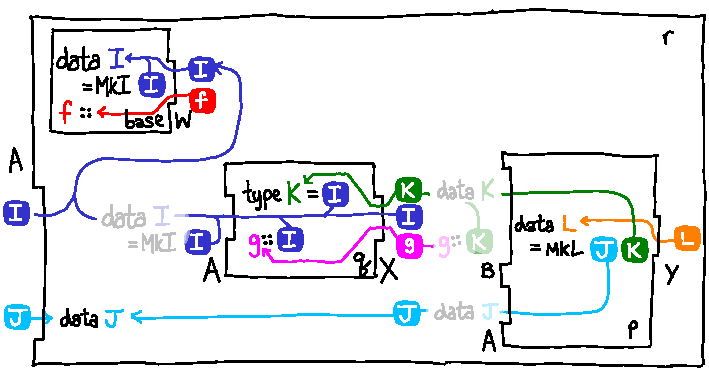
\includegraphics{figures/pqr-type-diagram.pdf}
\caption{Pictorial depiction of the types in our running example
(Figure~\ref{fig:linked-example}), with all original names replaced with
pointers to the declaration of the semantic object.
Lightened declarations (seen to the left of the holes for \texttt{A} and
\texttt{B} in \texttt{q} and \texttt{p}) specify requirements which
were subsequently filled by instantiation or signature merging.}
\label{fig:typing-example-diagram}
\end{figure}

After mixin linking has produced a \unit{} definition from a \ccomp{}
definition, the component can now be \emph{typechecked}, producing \emph{module types}
which record the type information
of all top-level declarations in a module.
GHC Haskell's module types resemble Haskell source code,
with two differences:
first, all declarations have been annotated with full type and kind
information; second, all identifiers have been renamed into \emph{original
names} which identify the exact module which originally defined the
entity.  The types of our running example can be found
in Figure~\ref{fig:typing-example}; to see the full grammar for module
types skip ahead to Figure~\ref{fig:semantic-objects}.

In the rest of this section, we'll describe the interface and semantic
representations in more detail, and outline how each type of declaration
in a \unit{} can be typechecked.

\subsection{Typechecking a module}

A module is typechecked to produce a \emph{module
type}, consisting of an \emph{export
specification} (what gets brought into scope when
you import this module) and a set of \emph{defined entity specifications}
(the types and values defined by this module).

%   Syntactically, these are represented with
%   a notation reminiscent of Haskell module declarations:
%   $\UobjTau{\UNs}{\overline{\Uty}}$.

For example, the module
\modname{W} in \cidl{base} (Figure~\ref{fig:linked-example}) type
checks to the following module type (see also Figure~\ref{fig:typing-example}):

\begin{figure}[H]
\center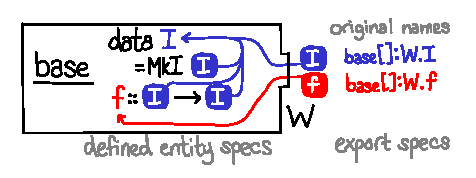
\includegraphics{figures/base-types.pdf}
\end{figure}

\noindent
In the diagram, we depicted the type of \verb|box| pictorially
by wiring up the enboxed references of \texttt{I} and \texttt{f} to their definitions.
The enboxed references \texttt{I} and \texttt{f} are
not unresolved Haskell-source level names,
but \emph{original names} $N ::=
M.n$, which serve as unique identifiers for any entities; in the
diagram, the original names have been abbreviated for concision.  An
original name for an entity defined in a module is generated by joining
the identity of the module that defines it---$\MOD{base}{}{W}$ in this
case--- with the Haskell source level name (e.g., \texttt{I},
\texttt{f}).
If, when typechecking another module, we need to look up the kind of
$\MOD{base}{}{W}.\texttt{I}$, we look up the module type of
$\MOD{base}{}{W}$ from the context and then find the defined entity
specification for \texttt{I} within the module type.

\subsection{Typechecking a signature}

Typechecking \cidl{q} (Figure~\ref{fig:linked-example}) from our running example requires
us to deal with a signature declaration.  Here is a
representation of the final type of \cidl{q}:

\begin{figure}[H]
\center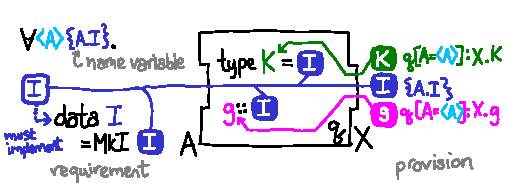
\includegraphics{figures/q-types.pdf}
\end{figure}

\noindent
In the diagram, the declarations from the signature are
drawn externally from \cidl{q}.  We do not know what module
will be used to fill the requirement \texttt{A}, and
consequently, we don't know what original name will provide an
implementation of \texttt{I}, although we do have a declarative
specification which any implementation must satisfy.  When we type check against the
signature, we use this required declaration ``as if'' it were
a declaration of its own.

In mixin linking, we bound a module variable \hv{A} to represent the
unknown module identifier.  In typechecking, we bind a \emph{name
variable} $\nhv{m.n}$ to represent the unknown entity $n$ required by
requirement $m$.
You may be wondering why name variables are not simply defined as
$\hv{m}.n$.  Read literally, names of this form demand that $n$ be defined
by $\hv{A}$ itself, ruling out the possibility that it \emph{reexports}
$n$ from another module.

In the diagram above, the results of typechecking the module \texttt{X}
are also shown.  As before, entities that are defined in the module
are given original names combining the module identifier (\MOD{q}{\subst{A}{\hv{A}}}{X})
and their source level name, while reexported entities retain the original
name of their source.

\subsection{Typechecking a dependency}

Now we can define the key operation for typechecking in \Backpack{}:
how to compute the type of \cidl{q} instantiated with an implementation
for its requirements.  These instantiations are specified to the
compiler via \textsf{dependency} declarations.
Let's first consider a simple one: filling \cidl{q}'s
requirement with \modname{W} from \cidl{base}, i.e., $\UsynDepEmpty{\cidl{q}[\subst{A}{\Mod{\cidl{base}[]}{W}}]}$.

\begin{figure}[H]
\center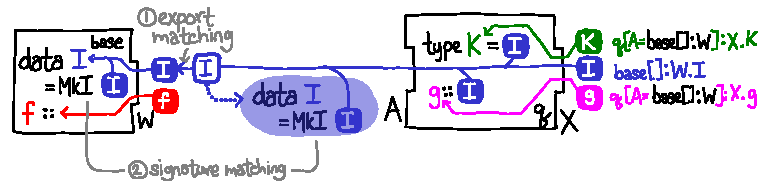
\includegraphics{figures/base-q-types.pdf}
\end{figure}

\noindent There are two key steps. First, we take the
required export specification from \cidl{q}, and the provided export
specification from \cidl{base}, and we perform \emph{export matching},
matching every required entity with an exported entity with the same
name from the implementing module.  In our example, we learn that
\nhv{A.I} is instantiated with \MOD{base}{}{W}.\texttt{I}; in the graph
representation, all previous references to \nhv{A.I} are rewritten so
that they now point to the declaration for \MOD{base}{}{W}.\texttt{I}.
Additionally, we must apply the module substitution to the original names of all
entities defined in the instantiated component: e.g., we apply the
substitution $\subst{A}{\Mod{\cidl{base}[]}{W}}$ to the original name
\MOD{q}{\subst{A}{\hv{A}}}{X}.\texttt{K}.

When we do this, we must check if this instantiation is
well-typed via \emph{signature matching}: do the
declarations provided by \cidl{base} match the required declarations of
\cidl{q}?  This proceeds by comparing the declarations of each required
entity with the declaration of the corresponding provided entity.
In our example, the implementation of \texttt{I} is an algebraic data
type which matches the required declaration exactly; the implementation
would also have successfully matched an abstract data type \texttt{data I}.

It is important that export matching happen before
signature matching, as the process of export matching may reveal more
type equalities.  This can be seen in the instantiation of \cidl{p} in
our running example:

\begin{figure}[H]
\center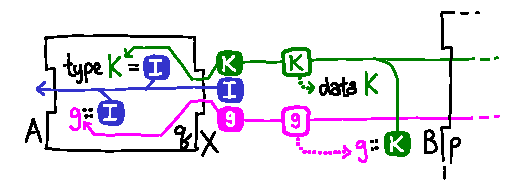
\includegraphics{figures/instantiation-with-synonyms.pdf}
\end{figure}

\noindent
In this example, it is not syntactically obvious that \verb|g :: I|
and \verb|g :: K| are matching declarations.  \verb|I|
and \verb|K| are definitionally equal because the abstract data type \verb|K|
was implemented by the type synonym \verb|type K = I|:

\begin{figure}[H]
\center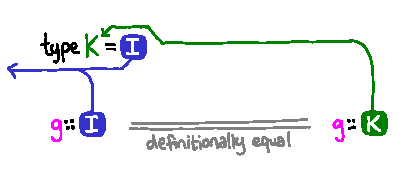
\includegraphics{figures/instantiation-with-synonyms-reduced.pdf}
\end{figure}

\noindent
By wiring up everything beforehand, we ensure that signature matching
sees the correct equalities.

%   This does mean that we may construct some
%   types in the graph representation that are ill-kinded before discovering
%   that signature matching fails!

\subsection{Signature merging}
\label{sec:signature-merging}

The distinguishing characteristic of mixin
linking is not just the linking that occurs when a module is brought into
scope with the same name as a signature, but also the \emph{signature merging}
that occurs when two signatures are brought into scope under the same name.
Like dependency instantiation, we must take the required exports of each
signature being merged and merge them with the identically
named entities from other signatures.

%   Unlike dependency instantiation,
%   this matching process is \emph{bidirectional}, as can be seen in the

The subtlety of signature merging is determining whether or not the declarations
of a type in two signatures are compatible with one another.  Consider
the following example (which is adapted from the MixML paper~\cite{rossberg+:mixml}):

\begin{tabular}{p{0.45\textwidth} p{0.45\textwidth}}
\begin{lstlisting}
signature A where
    type T = Int
    data U
    f :: Int -> U
\end{lstlisting}
&
\begin{lstlisting}
signature A where
    data T
    type U = Bool
    f :: T -> Bool
\end{lstlisting}
\end{tabular}

\noindent
It is not obvious that \verb|Int -> U| has the same type as \verb|T -> Bool|,
unless we refine \verb|U| to \verb|Bool| and \verb|T| to \verb|Int| in
both signatures.

\begin{figure}[H]
\center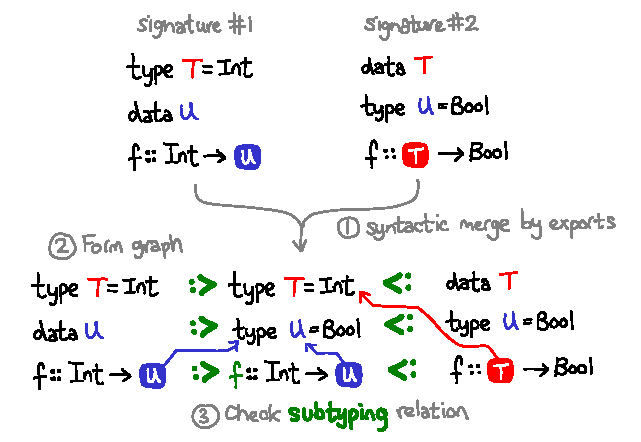
\includegraphics{figures/signature-merging.pdf}
\end{figure}

\noindent
To merge these signatures,
we first take the required export specifications from each signature and
match entities which have the same names.
For every entity which occurs in multiple signatures,
we pick out the most-defined
declaration from each signature.  In this example, the choice is easy:
\verb|type T = Int| is more defined than the abstract \verb|data T|,
so we pick it for the merged signature.
If there is not a unique choice, we pick an arbitrary one.

Then, we check if each of the original declarations are compatible with
the merged declaration.  The important twist is that whenever we
see a name in one of the original declarations, we must resolve it
to its definition in the \emph{merged} signature: in the diagram above,
this is depicted by pointing the enboxed references to the central
declarations.  Now we can see that both instance of \verb|f| have a type that
is definitionally equal to \verb|Int -> U|.

%   \paragraph{Signature merging}
%   There is one final detail: how to merge requirements from
%   the dependencies of a component.  If
%   we know the required module types of all our dependencies, the merge is
%   straightforward.  For example, here are the module types to be merged
%   in \cidl{r} for the signature \modname{A}:
%   \[
%   \begin{array}{lll}
%   &\begin{array}{l}
%       \UobjIface\: (\MOD{base}{}{W}.\texttt{I}) \\
%   \end{array} & \text{Local signature} \\
%   \oplus&
%   \begin{array}{l}
%       \UobjIface\: (\nhv{\texttt{A.J}}) \\
%       \quad\texttt{data J :: *}
%   \end{array} & \text{From \cidl{p}} \\
%   \oplus&
%   \begin{array}{l}
%       \UobjIface\: (\nhv{\texttt{A.I}}) \\
%       \quad\texttt{data I :: * = MkI}\ \nhv{\texttt{A.I}}
%   \end{array} & \text{From \cidl{q}} \\
%   =&
%   \begin{array}{l}
%       \UobjIface\: (\MOD{base}{}{W}.\texttt{I}, \nhv{\texttt{A.J}}) \\
%       \quad\texttt{data J :: *}
%   \end{array} & \text{Final requirement for \cidl{r}}
%   \end{array}
%   \]
%   %
%   The export lists are unioned together, and we discover that \nhv{A.I}
%   actually must implemented with $\MOD{base}{}{W}.\texttt{I}$. And since
%   the entity \texttt{I} is already implemented, we additionally
%   drop its specification from the resulting requirement (having checked
%   that its specification from \MOD{base}{}{W} matches that from \cidl{q}).

%   Unfortunately, this definition of signature merging is circular: to
%   compute the instantiated type of a component, we need to know the (full)
%   types of our requirements; but to compute the type of a merged
%   requirement, we need to compute the instantiated types of the components
%   which merge into the requirement. \Scott{I'm not sure what this means. Can
%   you identify how the problem manifests in the example so far?}
%   The solution to this problem is to
%   define \emph{partial instantiation}, which only instantiates a component
%   type as much as is necessary to determine the type of the requirement in
%   question.  We give the technical details in Section~\ref{sec:compiler}.

%   \paragraph{Compiling instantiated components}
%   \Red{Need to rewrite this section, motivate why the semantics split
%   into separate type checking and compiler.}
%   When a \unit{} has no
%   requirements, it can be compiled.  In this case, compilation is very
%   trivial: the dependencies of \unit{}s can be successively instantiated
%   by Cabal to form a graph of instantiated components, which GHC can
%   simply compile in order.  In this way, the soundness of Haskell with \Backpack{}
%   trivially reduces to the soundness of Haskell without \Backpack{}.

%   While compilation of \Backpack{} is trivially sound, we would like to
%   relate type checking and compilation with a property that says that if a
%   unit typechecks compositionally, it also typechecks monolithically
%   (i.e., when you re-typecheck the entire transitive closure.)
%   Unfortunately, in full Haskell it is impossible for this to be the case
%   with our current signature language and semantics.  In Section \Red{XXX}
%   we give some examples and conjecture under what circumstances this
%   property does hold.


\section{Instantiation and compilation}
\label{sec:overview-instantiate}

Typechecking is all very well and good, but what about
running our programs?  For both soundness reasons (Section~\ref{sec:limitations})
and performance reasons, it is desirable to defer compiling
until we know how all the requirements of a component are to be
filled.

When we have a \unit{} which has no unfilled requirements,
the package manager computes the
\emph{instantiated component graph}, reflecting all of the
concrete code dependencies of the component.  Specifically, given a closed instantiated component identity $p[S]$, for every
\textsf{dependency} $P$ of $p$'s mixed component, recursively
instantiate $\substw{P}{S}$.  Furthermore, for every $\substMod{m}{P}{m'} \in S$,
recursively instantiate $P$.  Then, we compile each instantiated component
in topological order.  This compilation is exactly like ordinary
compilation without \Backpack. The only new feature is that signatures
compile into trivial module which reexport entities from
the backing implementation; otherwise, modules that imported the signature might see
entities from the backing implementation that were not exported by the
signature.

It is important that the package manager computes
the instantiated component graph: \emph{applicative}
semantics of instantiation mean that completely independent
components could instantiate a library in the same way: in such
cases we should share the compiled code.  A traditional compiler cannot
do this: it is solely responsible for transforming source
files into object code.











%%% Local Variables:
%%% mode: latex
%%% TeX-master: "paper"
%%% End:
